\section{Aufbau und Durchführung}
Der erste Schritt bestand darin, das Programm zu schreiben, welches den Messvorgang steuert, also Magnetfeld hoch- und runterfährt, sowie Messwerte ausliest und in einer Datei speichert. Dazu wurde LabView verwendet.

\subsection{Magnetotransportmessung}\label{sec:Magnetotransport}
Bei diesen Messungen geht es darum, die Magnetotransporteigenschaften der Probe zu bestimmen.

\begin{wrapfigure}[13]{r}{7.5cm}

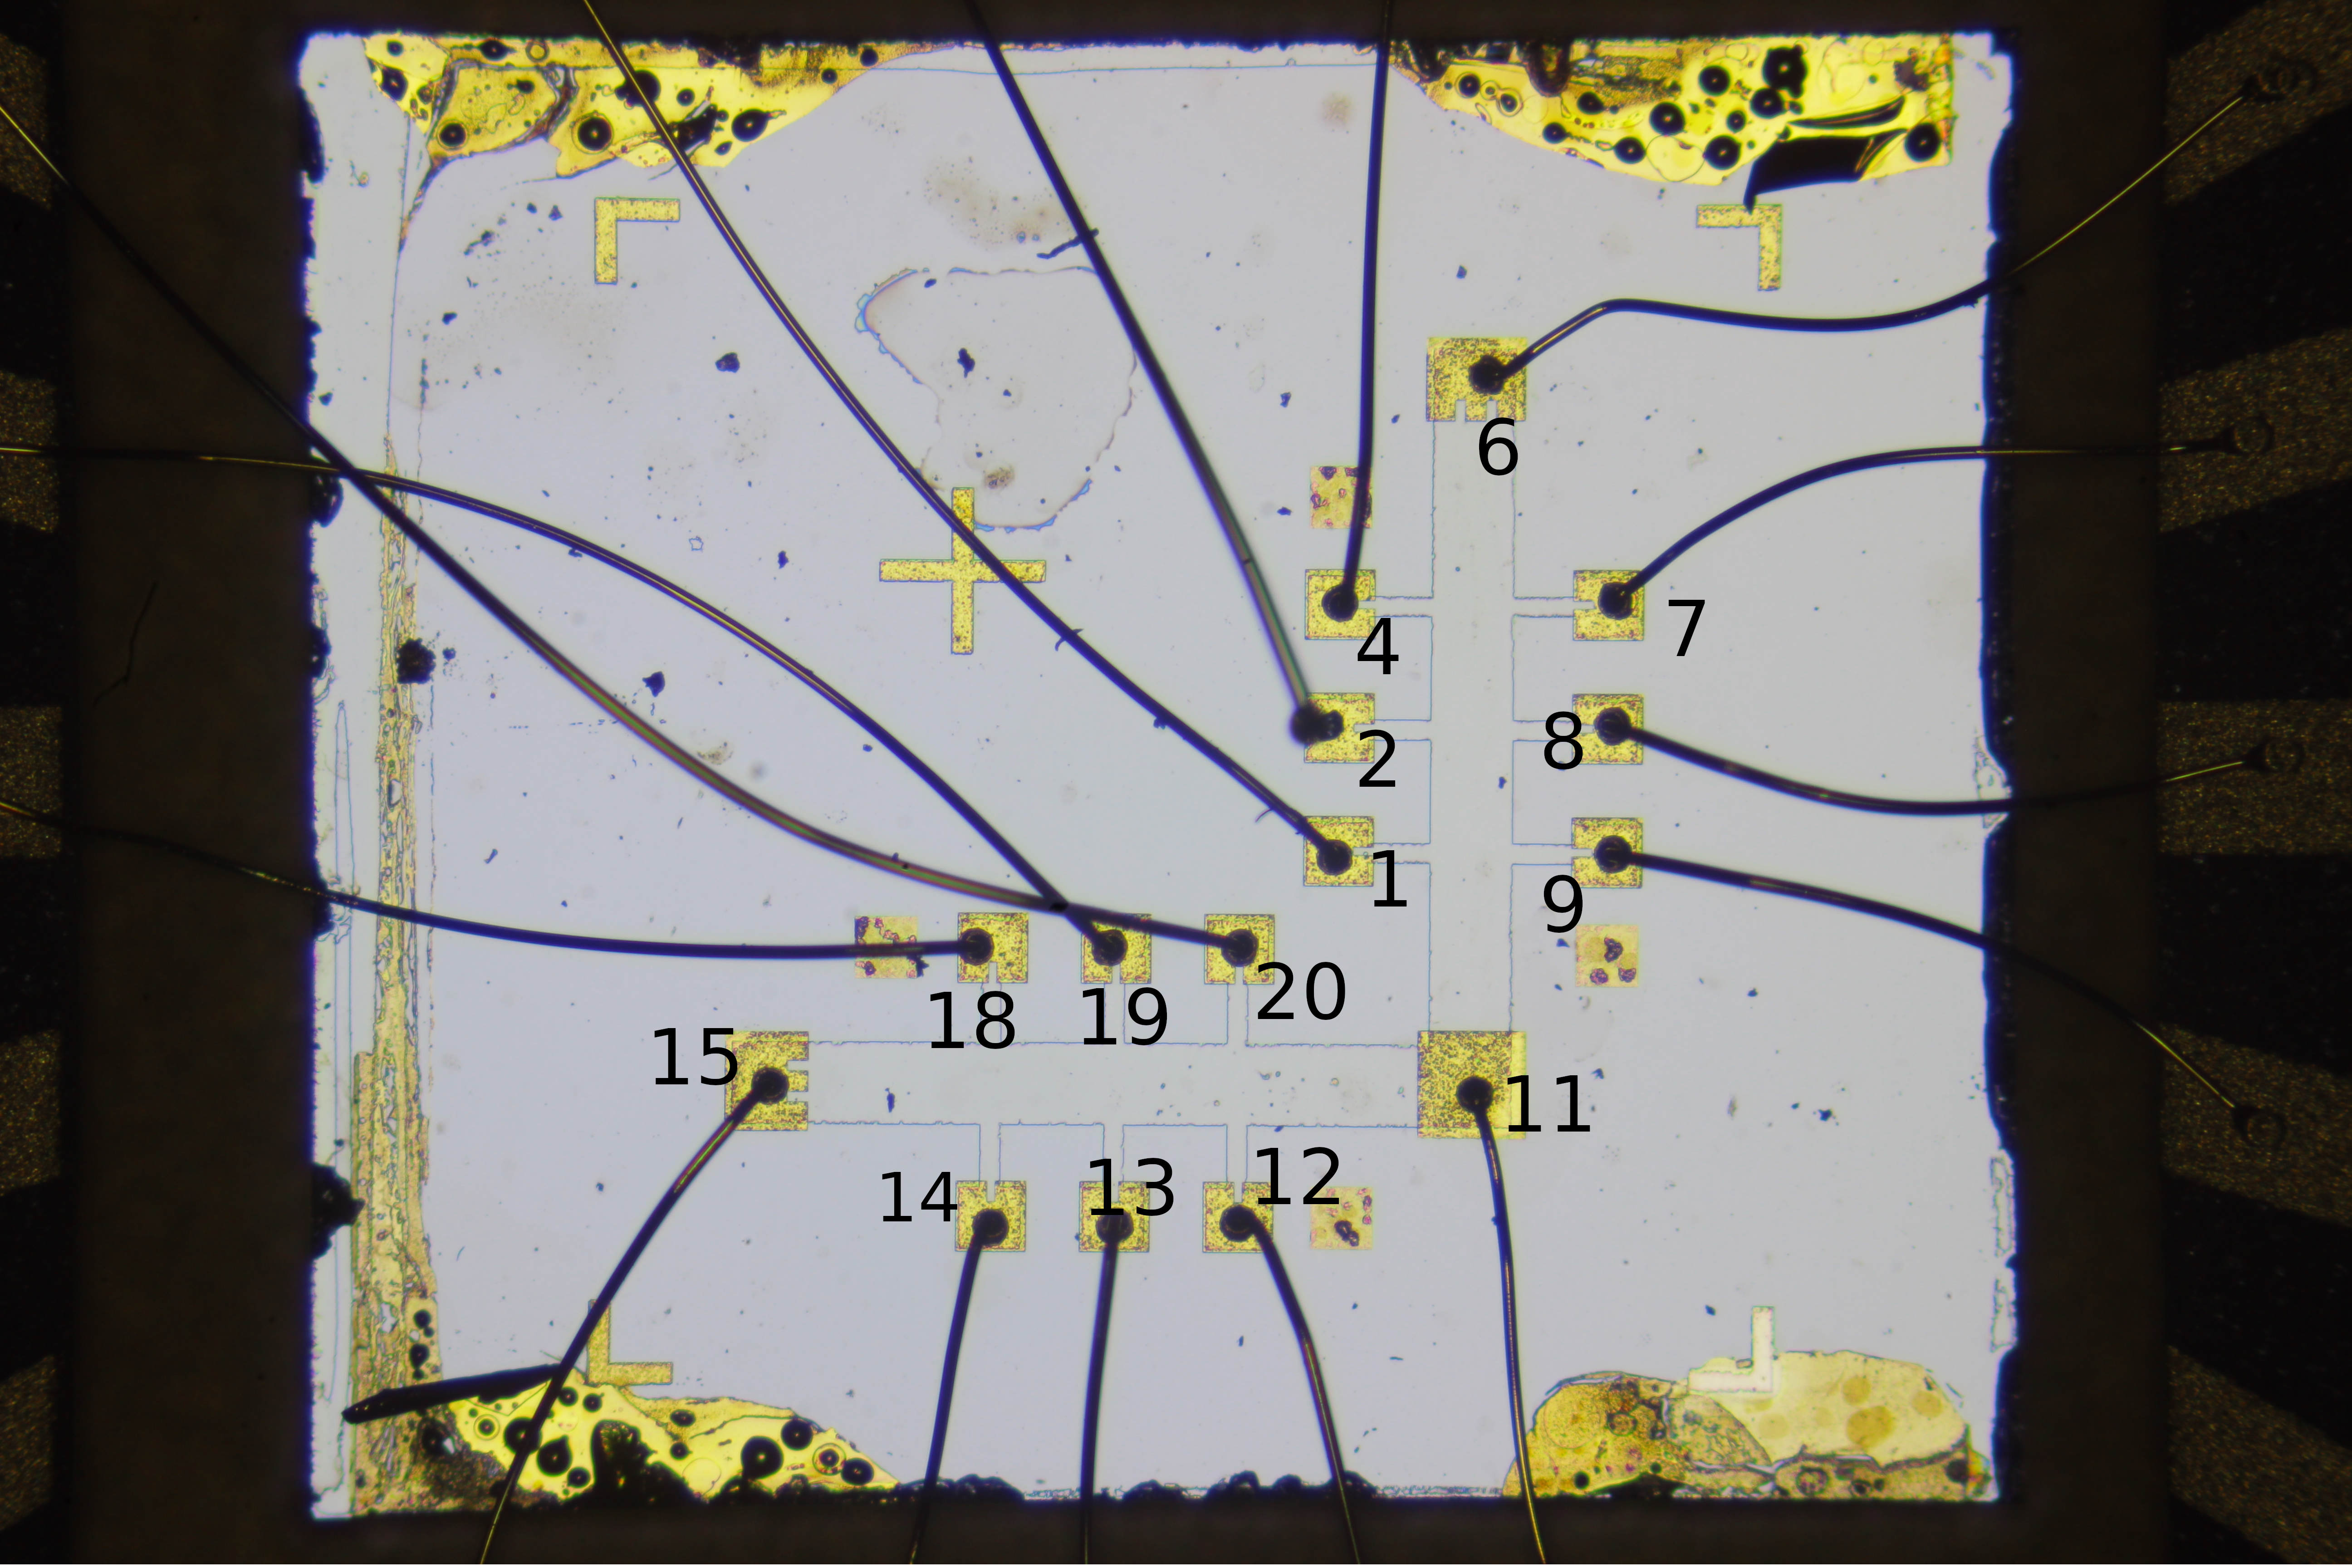
\includegraphics[scale=0.04]{Pictures/P07BondSchema.jpg}
\caption{Bond-Schema von Probe \emph{P07}}

\label{fig:P07}

\end{wrapfigure}
\hfill\\
Der Magnetprobenstab, an dessen unteren Ende sich eine Spule befindet, wird in der Heliumkanne platziert.
Die Probe (\emph{P07}, Bond-Schema siehe \autoref{fig:P07}) wird in den Probenstab eingesetzt und dieser wiederum in den Magnetprobenstab eingelassen.
Vor der ersten Messung muss lange genug gewartet werden, sodass die eingebrachten Bauteile abkühlen können.\\
Über ein Schaltbrett, das es erlaubt, auf die verschiedenen Kontakte der Hallgeometrie zuzugreifen, wird der Stab mit einer Stromquelle (\emph{Keithley 2400}) verbunden.
Zum Aufbauen des Magnetfelds wird ein weiteres Netzteil benötigt.
Mittels zweier \emph{Keithley 2000} werden Längs- und Querspannung gemessen.\\\\
Dabei wird der Längsstrom von $10\ \si{\micro A}$ an zwei verschiedene Kontaktpaare angelegt.
Für jedes Kontaktpaar werden die Spannungsmessgeräte wiederum mit jeweils zwei Kontaktpaaren verbunden, sodass vier Messreihen entstehen.
In jeder Messreihe wird das Magnetfeld von $0\ \si{T}$ auf $4\ \si{T}$ hochgefahren (oder andersherum) und in geeigneten Abständen werden Längs- und Querspannung aufgenommen.
Die Kontaktpaare sollen nach Möglichkeit verschieden sein, was jedoch aufgrund defekter Kontakte nicht immer uneingeschränkt möglich war.\\
Aus den Messwerten werden dann Elektronenkonzentration und -beweglichkeit bestimmt.\\\\
Die verwendeten Paarungen (inklusive den in \autoref{sec:Auswertung} verwendeten Bezeichnungen der Messreihen) sind in \autoref{tab:PairsP07} zu finden.\\

\begin{table}[ht]
\caption{Für die Messungen zum Magnetotransport verwendete Kontaktpaarungen}
\label{tab:PairsP07}
\centering
\begin{tabular}{cccc}
\toprule
Bezeichnung & Strom & Längswiderstand & Hallwiderstand\\
\midrule
P07\_1\_A & $6\rightarrow 11$ & $7\rightarrow 8$ & $1\rightarrow 9$\\
P07\_1\_B & $6\rightarrow 11$ & $7\rightarrow 9$ & $1\rightarrow 9$\\
P07\_2\_A & $11\rightarrow 15$ & $12\rightarrow 13$ & $20\rightarrow 12$\\
P07\_2\_B & $11\rightarrow 15$ & $20\rightarrow 18$ & $19\rightarrow 13$\\
\bottomrule
\end{tabular}
\end{table}
\subsection{Dauerhafter Photoeffekt}\label{sec:Photoeffekt}
Bei sehr tiefen Temperaturen kann der durch den Photoeffekt erzeugte Strom auch nach Ausschalten der Beleuchtung noch gemessen können.
Dies soll anhand dieser Messungen verifiziert werden.

\begin{wrapfigure}[13]{r}{7.5cm}
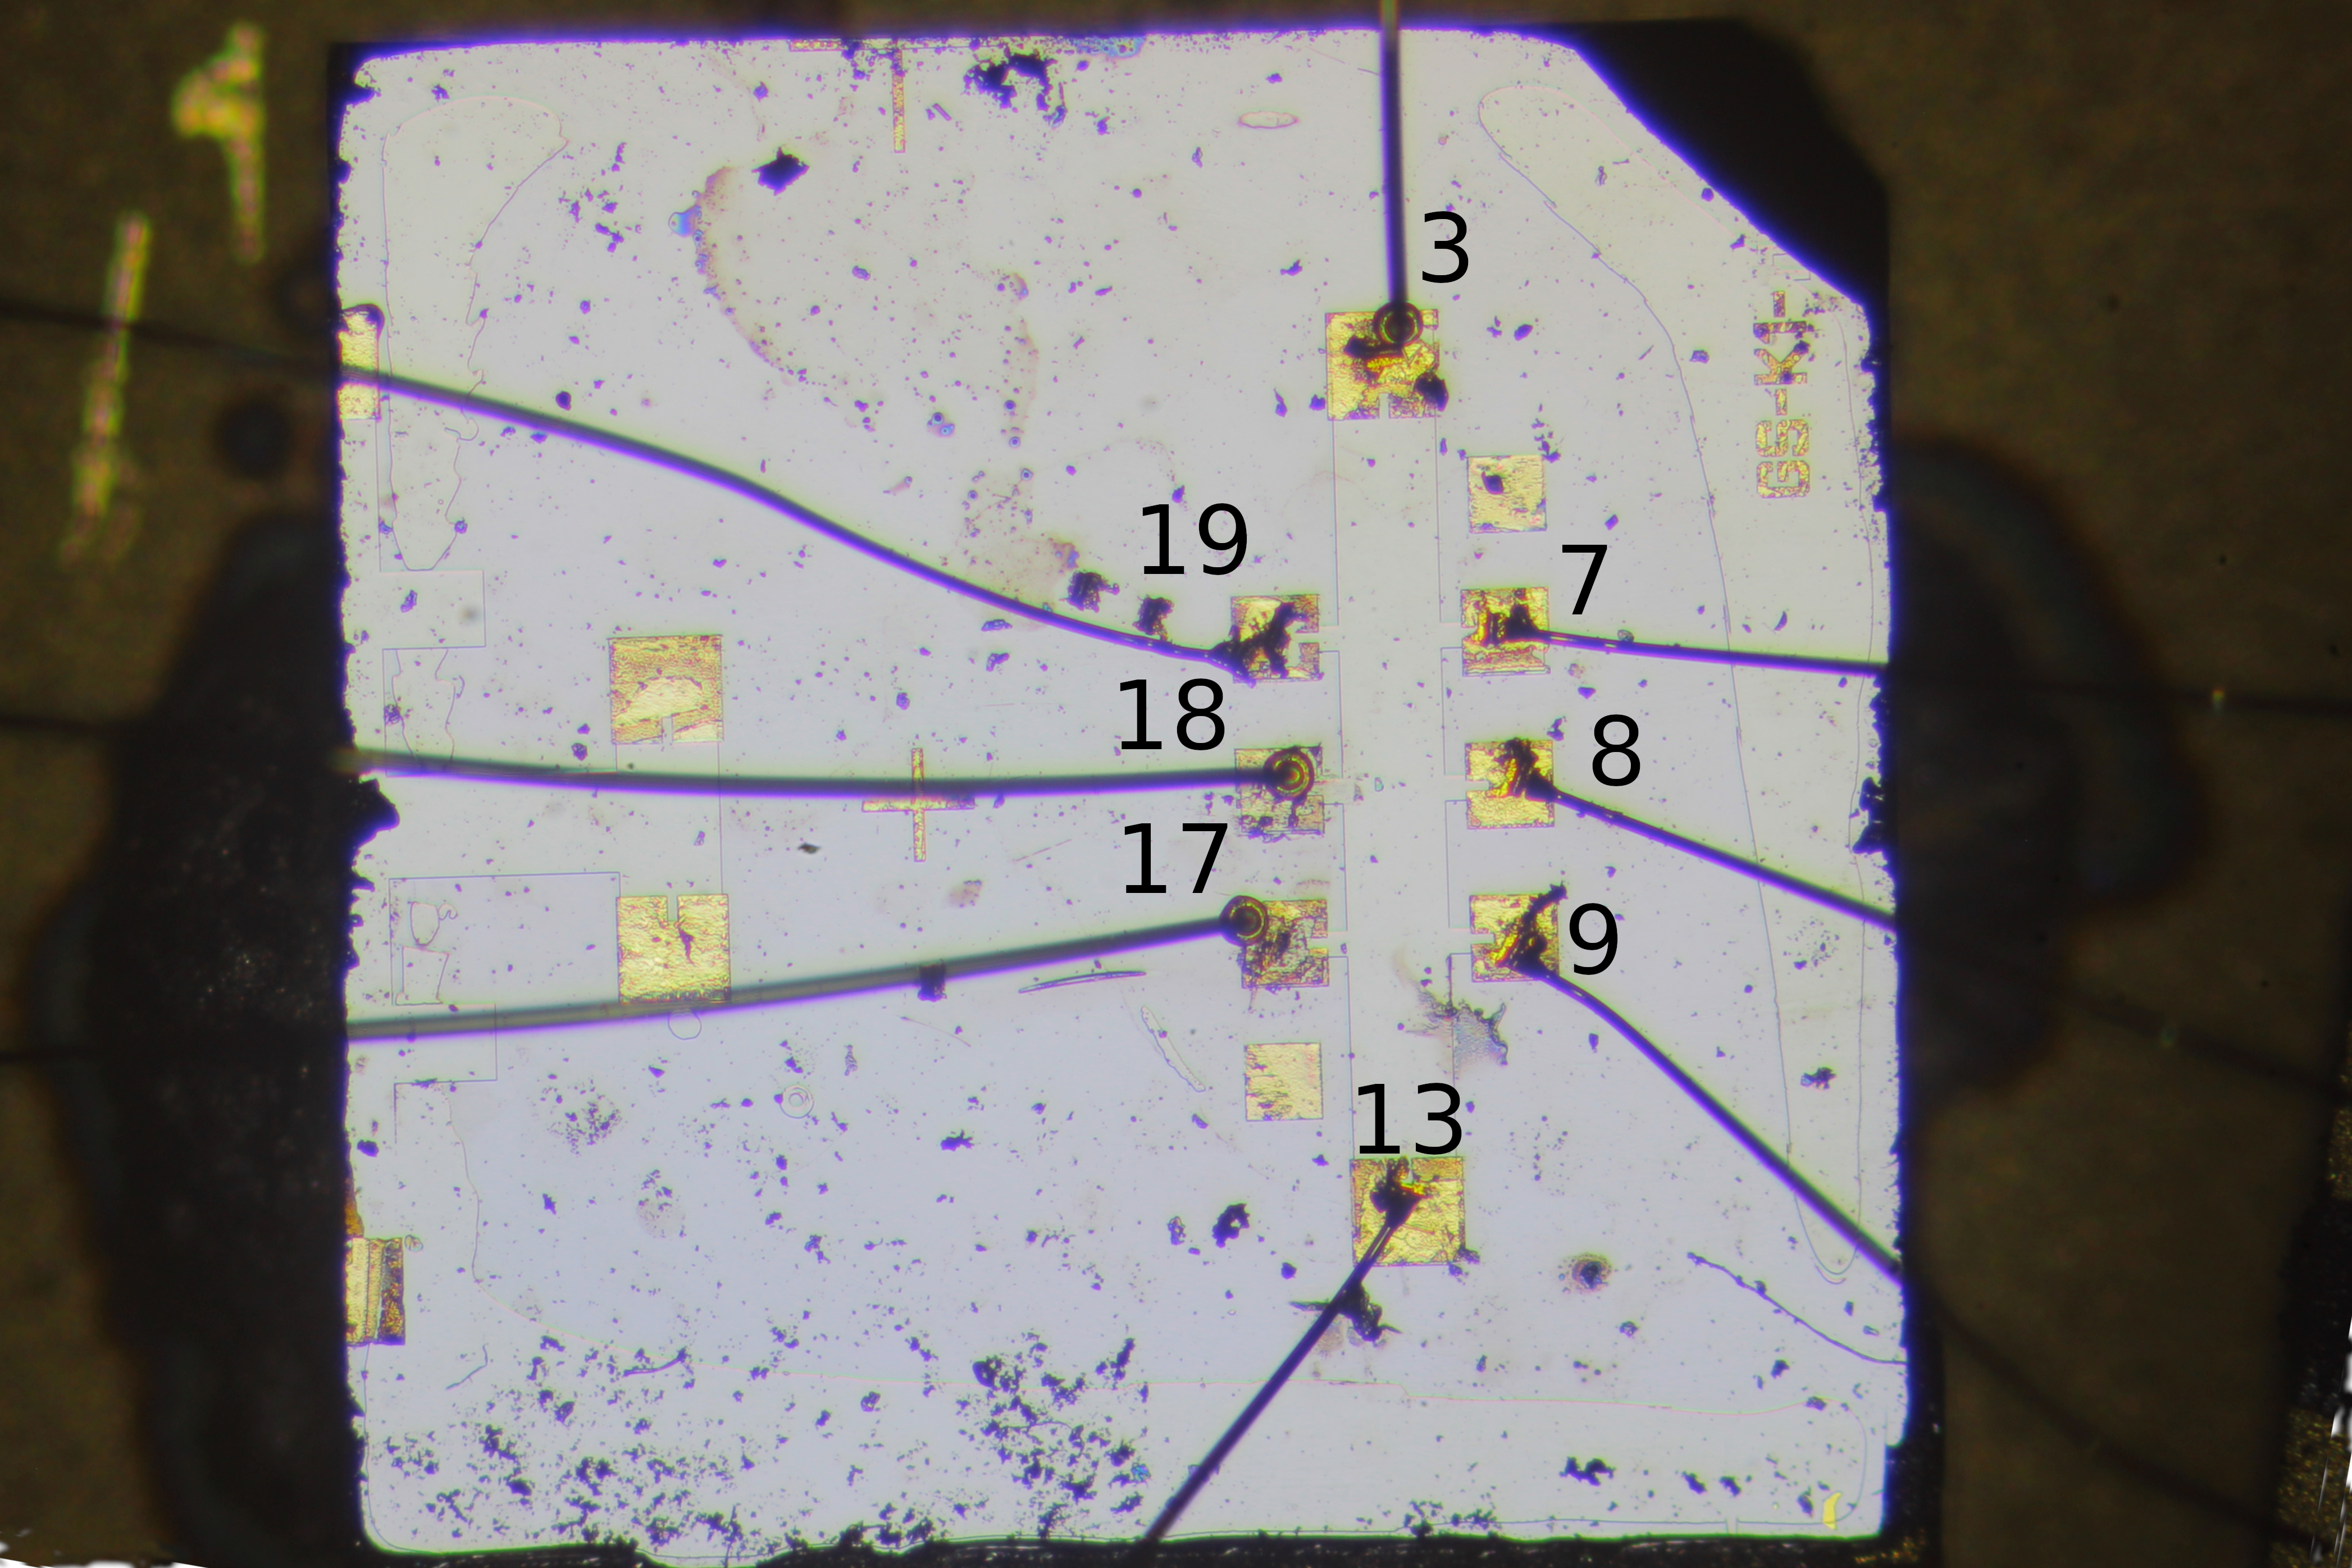
\includegraphics[scale=0.05]{Pictures/P04BondSchema}
\caption{Bond-Schema von Probe \emph{P04}}
\label{fig:P04}
\end{wrapfigure}
\hfill\\
Der Aufbau der Messung ist zum größten Teil identisch zu dem in \autoref{sec:Magnetotransport} beschriebenen. Es wird jedoch eine andere Probe (\emph{P04}, Bond-Schema siehe \autoref{fig:P04}) verwendet, auf welcher außerdem eine LED angebracht wird.

Bei diesen Messungen wird der Strom stets an dieselben Kontakte angelegt.
Zunächst werden für zwei Kombinationen von Kontakten Messungen analog zu \autoref{sec:Magnetotransport} durchgeführt. Die verwendeten Paarungen sind \autoref{tab:PairsP04} zu entnehmen.\\
Anschließend wird mit einem \emph{Keithley 2400} an die LED ein Strom von $8\ \si{mA}$ angelegt und die Probe für $60$ Sekunden beleuchtet.
Nach einer Wartezeit von zehn Minuten wird die Messung wiederholt.\\
Elektronenkonzentration und -beweglichkeit werden berechnet und verglichen.

\begin{table}[ht]
\caption{Für die Messungen zum Magnetotransport verwendete Kontaktpaarungen}
\label{tab:PairsP04}
\centering
\begin{tabular}{cccc}
\toprule
Bezeichnung & Strom & Längswiderstand & Hallwiderstand\\
\midrule
P04\_1 & $3\rightarrow 13$ & $7\rightarrow 8$ & $19\rightarrow 7$\\
P04\_2 & $3\rightarrow 13$ & $19\rightarrow 17$ & $17\rightarrow 9$\\
\bottomrule
\end{tabular}
\end{table}
